\blue{
\begin{itemize}
\item Broader context
    \begin{itemize}
    \item UK energy production and usage. Climate crisis, fuel switching and nuclear. Why is combustion so important even with nuclear? Hydrogen is another option. But [for reasons] is more susceptible to thermoacoustic instab. 
    \end{itemize}
\item Motivation for the PhD
    \begin{itemize}
    \item combustion instabilities
    \item porous media/complex geometries
    \item connections to other instabilities
    \end{itemize}
\item Motivation for this year's work
    \begin{itemize}
    \item Expensive TA simulations usually
    \end{itemize}
\item In last year's report
    \begin{itemize}
    \item Explored the hydrodynamic model for flames and models derived therein, particularly the Markstein model and Michelson-Sivashinsky model
    \end{itemize}
\item Report structure / 'in this report we...'
    \begin{itemize}
    \item perform a lit review. discuss the numerical methods and techniques used. introduce the idea for delay BCs and implement them into an existing software. provide results and discussion. plan upcoming years of the phd
    \end{itemize}
\end{itemize}
}


\begin{figure}[t]
\centering
    \begin{subfigure}{0.40\textwidth}
    \centering
    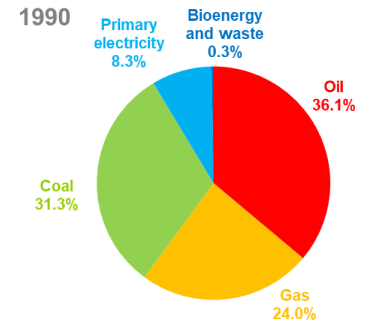
\includegraphics[height=5cm]{assets/graphs/energy-consumption_1990.png}
    \end{subfigure}
    \begin{subfigure}{0.40\textwidth}
    \centering
    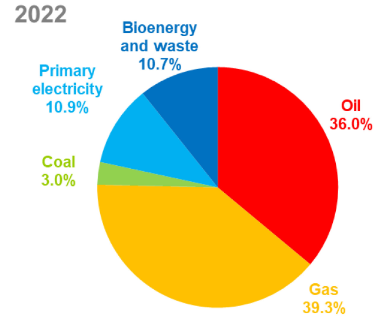
\includegraphics[height=5cm]{assets/graphs/energy-consumption_2022.png}
    \end{subfigure}
\caption{Total energy production in the United Kingdom in 1990 and 2022 \cite{departmentforenergysecurityandnetzero2023UKEnergyBrief}.}
\label{fig:fuel-consump}
\end{figure}

The growth of international populations and industry have meant that the global market for energy is higher than ever \cite{newell2019GlobalEnergyOutlook} and the reliance on fossil fuels is ubiquitous despite international efforts to quell the emission of carbon into the atmosphere \cite{unitednations2015ParisAgreementUNFCCC}. Nevertheless, with the price of green energy at its lowest historical levels \cite{internationalrenewableenergyagency2022RenewablePowerGeneration} and the threat of irreversible climate crises imminent, work must be done to adopt renewable energy sources. In Britain, the removal of coal as an energy source was successful, as shown in \fig{fig:fuel-consump}. This \emph{fuel switching} from coal to gas and oil, promoted by effective economic factors, led to a 6\% decrease in the country's overall carbon emissions despite an increase in overall energy consumption \cite{wilson2018RapidFuelSwitching}. With natural gas, methane is almost exclusively burnt, and the domestic and industrial sectors account for approximately a third each (237 TWh and 206 TWh of methane, respectively) of the total methane consumption in Britain in 2023 \cite{departmentforenergysecurityandnetzero2023HistoricalGasData}.

One appropriate renewable source of energy is that of hydrogen, which is unlikely to replace the usage of fossil fuels but may be used alongside gas in applications where gas was already being burnt \cite{momirlan2005PropertiesHydrogenFuel}. Combustion of hydrogen with air is usually performed lean to avoid the NO$_x$ pollution risk under stoichiometric hydrogen-air combustion. Although lean hydrogen combustion is greener than gas or oil, different hydrogen production processes \cite{dasilvaveras2017HydrogenTrendsProduction} cause significant variations in carbon emissions \cite{nationalgrid2022HeatingOurHomes}. Hydrogen represents an attractive energy source \cite{momirlan2005PropertiesHydrogenFuel}, particularly through fuel cells \cite{momirlan2005PropertiesHydrogenFuel} and combustion \cite{lanz2001Module3Hydrogen, stepien2021ComprehensiveOverviewHydrogenFueled}. The combustion of hydrogen in particular may be used for internal combustion engines, gas turbines cookers and gas boilers \cite{momirlan2005PropertiesHydrogenFuel}. It has also been estimated that by 2040, the demand for hydrogen in the United States will have grown to 15 million tons \cite{molkov2007HydrogenSafetyResearch} and represents the growth of the \emph{hydrogen economy}.

Hydrogen presents significant safety concerns \cite{green2006HydrogenSafetyIssues} especially in its gaseous form, with an obvious example of this being the 1937 Hindenburg disaster \cite{dilisi2017HindenburgDisasterCombining}. One probable cause being the light H\sub{2} molecules escaping the Zeppelin and catching alight. Beyond this, lean hydrogen-air combustion is subject to two primary instabilities which pose challenges to engineering applications. The high mass diffusion of hydrogen results in significant \emph{thermodiffusive instabilities}, where the flame spontaneously wrinkles and curves, forming many small cellular structures \cite{sivashinsky1983InstabilitiesPatternFormation} and massively increasing the speed of mass hydrogen consumption \cite{howarth2023ThermodiffusivelyUnstableLeanPremixed}. Lean hydrogen-air combustion also has an acute sensitivity to \emph{thermoacoustic instabilities}, where perturbations heat release from the flame couple to the acoustic modes of the combustor geometry, resulting in feedback. This can cause significant damage to combustors due to the extra mechanical work being done \cite{morgans2024ThermoacousticInstabilityCombustors}. Beyond these, the \emph{Darrieus-Landau instability} (also known as DL or hydrodynamic instability) is an intrinsic property of premixed flames which all are subject to, but pose little threat on their own to combustion applications as the resulting flames are attracted to a steady. albeit wrinkled, state \cite{matalon2018DarrieusLandauInstability}.

Of particular interest are how these fuels behave in complex geometries, especially for the purposes of porous media combustion (PMC). The benefits and applications of PMC are wide-reaching: PMC enables more effective transfer of heat from the combustion reaction to combustor \cite{mujeebu2009CombustionPorousMedia}; hydrogen combustion in PMCs enable leaner combustion \cite{tseng2002EffectsHydrogenAddition}; PMC has been used on the smallest scales, including in micro thermophotovoltaic systems \cite{pan2015HydrogenOxygenPremixed}; and PMC has been used for the passive control of the aforementioned thermoacoustic instabilities \cite{meadows2015PorousInsertsPassive, dowd2018ThermoacousticInstabilityModel}. Analytic studies form the foundation of instability research and provide many predictions for flames in simple geometries, but fall short in the case of these complex geometries. The next tool in our tool belt is Direct Numerical Simulation (DNS), where the fluid is fully resolved \cite{orszag1970AnalyticalTheoriesTurbulence}. The hydrodynamic and thermodiffusive instabilities are intrinsic to premixed flames and as such can be studied my performing DNS in the small region around the flame, so full combustor geometry need not be modelled to get an accurate understanding of their nonlinear behaviour. On the other hand, thermoacoustic instabilities besides the recently discovered intrinsic thermoacoustic modes \cite{silva2023IntrinsicThermoacousticInstabilities} require spatially modelling of the very small scale chemical processes as well as the large scale combustor geometry and temporally are bottlenecked by the speed of the implied acoustic waves. The motion of the flame within this combustor poses an additional challenge as some form of adaptive methods are typically required to accurately discretise the flame region. In practice, this makes it prohibitively expensive to perform DNS of full thermoacoustically unstable flames in, e.g. engines and so cheaper methods like large eddy simulation (LES) and Reynolds-averaged Navier-Stokes (RANS) are used which compromise accuracy in the flame region to render the large scale acoustics.

In last years report, we performed a holistic review of combustion and flame instabilities especially as they relate to hydrogen combustion. As background, the combustion equations were introduced alongside reasoning for the model assumptions made therein. Simplifications were made to show how these equations can be simplified into something more mathematically tractable. Details of numerical methods used to perform DNS were only briefly discussed. Initial findings given into the hydrodynamic instability and how successful qualitative models like the Michelson-Sivashinsky equation \cite{sivashinsky1977NonlinearAnalysisHydrodynamic, michelson1977NonlinearAnalysisHydrodynamic} fail to quantitatively match the flame shape for a unity Lewis number flame were given. A spectral solver was developed to more accurately model the flame in the case of high heat release, but this failed to account for non-negligible tangential velocities.


% The main objectives of this report are to perform a holistic literature review of relevant work and to show evidence of initial findings related to the PhD topic. \chap{ch:background} presents the governing combustion equations and present simplifications which can be made to formulate a simpler, mathematically tractable system of equations. On top of this, the Rankine-Hugoniot jump conditions and method of lines are presented as prerequisite knowledge for the coming chapters. This is followed by \chap{ch:lit_review} which constitutes the plurality of the report's contents and provides a literature review of the theoretical and experimental studies into the thermodiffusive, hydrodynamic and thermoacoustic premixed combustion instabilities. Initial findings are then given in \chap{ch:orig_work}, where we use a mesh-free combustion DNS code developed in \cite{king2022HighOrderSimulationsIsothermal, king2024MeshFreeFrameworkHighOrdera, king2020HighOrderDifference, kingSunsetFlames} to simulate hydrodynamically unstable flames in a simple periodic geometry. This is compared against the hydrodynamic theory of flames covered in \chap{ch:lit_review} and in particular to the Michelson-Sivashinsky equation which predates this theory. A spectral solver for the Michelson-Sivashinsky equation is also developed, but is found to be insufficient in the case of high heat releases and negligible tangential velocities. Finally, conclusions relating to this report are drawn in \chap{ch:conc} and \chap{ch:plan} organises a plan for the work proceeding this report.




